\documentclass[11pt,titlepage]{article}
\usepackage{fullpage}
\usepackage{amsmath}
\usepackage{amssymb}
\usepackage{color}
\usepackage{graphicx}
\graphicspath{ {images/} }
\usepackage{tikz}
\usetikzlibrary{shapes,arrows,positioning,calc}
\usepackage{float}
\restylefloat{table}
\usepackage{array}
\tikzset{
    block/.style = {draw, fill=white, rectangle, minimum height=3em, minimum width=3em},
    sum/.style = {draw, fill=white, circle, node distance=1cm},
    input/.style = {draw=none},
    output/.style = {draw=none},
    coord/.style = {coordinate}
}

\author{Rane Brown \\ Kate Schneider}
\title{ECEN 4638: Lab X.1PI}
\date{\today}

\begin{document}
\maketitle
\tableofcontents
\listoffigures
\newpage

\section{Description}
    This lab will further explore the Torsional Disc System. The system setup will be similar to what was used in labX.1P; only the bottom disc of the TDS will used and the four weights will be set at a radius of 6.5cm.

\section{System Model}
    \subsection{Calculated Parameters}

    \subsection{Transfer Functions}

\section{Matlab Analysis}\label{sec:mat_anys}
    \subsection{Time Domain}

    \subsection{Frequency Domain}

\section{Experimental Analysis}
    After conducting the matlab analysis in section \ref{sec:mat_anys} experimental data was collected from two different torsion disc systems. Data was collected from two systems in order to examine the robustness of the PI controller and make any necessary adjustments.
    \subsection{Setup}
    The first step in collecting experimental data was to select a rise time ($t_r$) and overshoot ($M_p$) for the system. As an initial starting point values of $t_r = 0.5$ sec and $M_p = 5\%$ were selected. Using these values the damping $\zeta$ and natural frequency $\omega_n$ were calculated using equations \ref{eq:zeta} and \ref{eq:omega}
    \begin{align}
        \zeta &= \frac{|\ln(0.05)|}{\sqrt{\pi^2+[ln(0.05)]^2}} = 0.69 \label{eq:zeta} \\[1em]
        \omega_n &= \frac{1.8}{0.5} = 3.6 \label{eq:omega}
    \end{align}
    These values were used as an initial starting point and adjustments were made based on the response calculated in matlab and the corresponding response on the TDS. In cases where the overshoot became too high the damping was increased. It also became necessary to increase the bandwidth of the system in order to reduce the noise on the live system. Table \ref{table:respData} shows the various calculated values based on necessary changes. For each iteration the value in bold was adjusted to improve the response. The adjustments were determined based on the response of the system to a step input as outlined in section \ref{sub:step} and to a ramp disturbance in section \ref{sub:dist}.
    \begin{table}[H]
        \centering
        \begin{tabular}{|m{1.5cm}|m{1.5cm}|m{1.5cm}|m{1.5cm}|m{1.5cm}|m{1.5cm}|m{1.5cm}|m{1.5cm}|} 
            \hline
            Test & $M_p$ & $t_r$ & $\zeta$ & $\omega_n$ & $K_p$ & $K_I$ & $BW$ \\ 
            \hline
            test1 & \textbf{5.00} & \textbf{0.50} & 0.69 & 3.60 & 0.1548 & 0.4611 & 6.55 \\
            \hline
            test2 & 19.58 & 0.090 & 0.69 & \textbf{10} & 0.469 & 3.558 & 19.55 \\
            \hline
            test3 & 16.23 & 0.085 & \textbf{0.80} & 10 & 0.5472 & 3.558 & 20.948 \\
            \hline
            test4 & 14.67 & 0.039 & \textbf{0.90} & \textbf{20} & 1.258 & 14.23 & 45.59 \\
            \hline
            test5 & 13.63 & 0.038 & \textbf{0.95} & 20 & 1.329 & 14.23 & 47.00 \\
            \hline
            test6 & 13.92 & 0.025 & 0.95 & \textbf{30} & 2.006 & 32.018 & 71.08 \\
            \hline
        \end{tabular}
        \caption{System Response} \label{table:respData}
    \end{table}

    \subsection{Time Domain - Step Response} \label{sub:step}
    The values shown in table \ref{table:respData} were calculated from the closed loop transfer function of the system model. The ideal step response from matlab was then compared to experimental data from the TDS. This experimental data was collected by adjusting the $K_p$ and $K_I$ values in Labview and saving the response data to a text file.\textcolor{red}{reference to transfer function or system model}. Data was collected for TDS machine 1 and TDS machine 4.
    \begin{figure}[H]
        \centering
        \begin{minipage}{.5\textwidth}
            \centering
            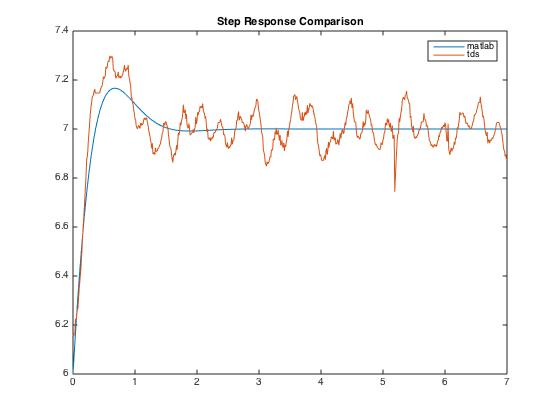
\includegraphics[scale=.4]{stepM1_T1}
            \caption{Step Response m1t1}
            \label{fig:stepM1_T1}
        \end{minipage}%
        \begin{minipage}{.5\textwidth}
            \centering
            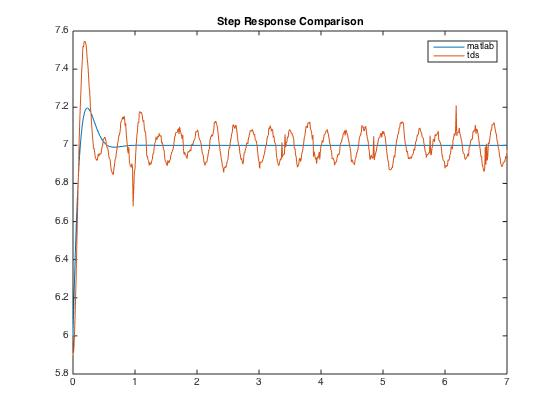
\includegraphics[scale=.4]{stepM1_T2}
            \caption{Step Response m1t2}
            \label{fig:stepM1_T2}
        \end{minipage}%
    \end{figure}
    \begin{figure}[H]
        \centering
        \begin{minipage}{.5\textwidth}
            \centering
            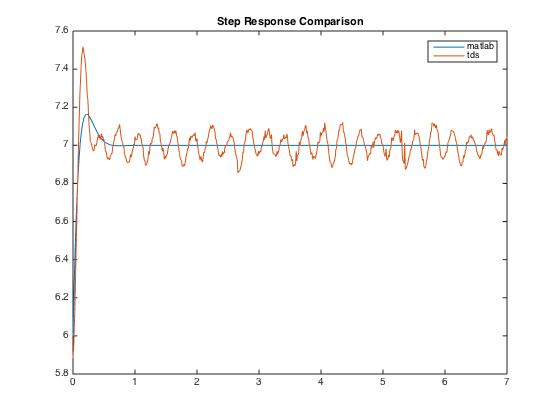
\includegraphics[scale=.4]{stepM1_T3}
            \caption{Step Response m1t3}
            \label{fig:stepM1_T3}
        \end{minipage}%
        \begin{minipage}{.5\textwidth}
            \centering
            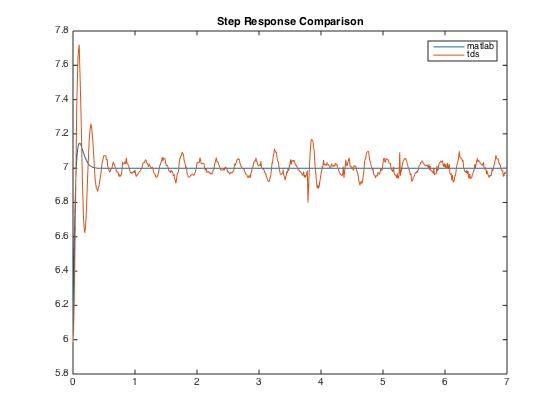
\includegraphics[scale=.4]{stepM1_T4}
            \caption{Step Response m1t4}
            \label{fig:stepM1_T4}
        \end{minipage}%
    \end{figure}
    \begin{figure}[H]
        \centering
        \begin{minipage}{.5\textwidth}
            \centering
            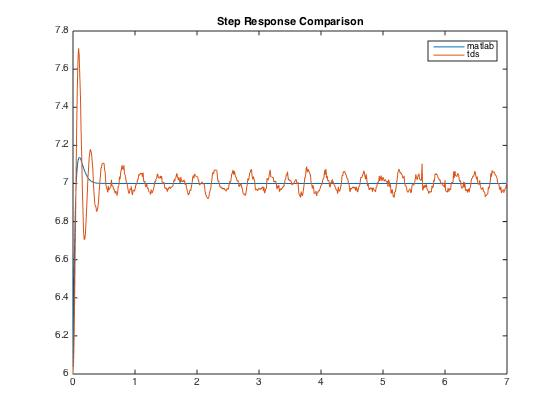
\includegraphics[scale=.4]{stepM1_T5}
            \caption{Step Response m1t5}
            \label{fig:stepM1_T5}
        \end{minipage}%
        \begin{minipage}{.5\textwidth}
            \centering
            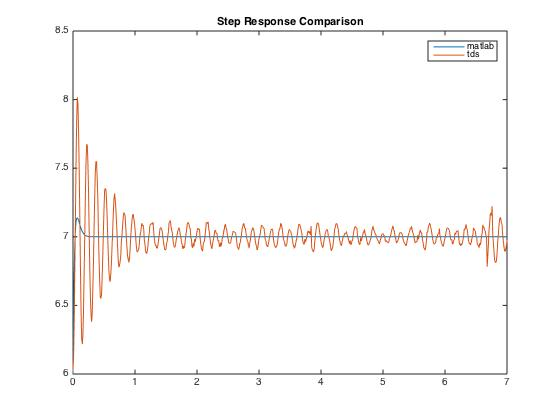
\includegraphics[scale=.4]{stepM1_T6}
            \caption{Step Response m1t6}
            \label{fig:stepM1_T6}
        \end{minipage}%
    \end{figure}
        \begin{figure}[H]
        \centering
        \begin{minipage}{.5\textwidth}
            \centering
            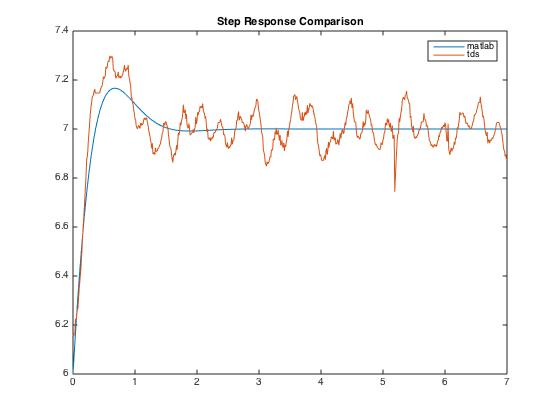
\includegraphics[scale=.4]{stepM1_T1}
            \caption{Step Response m1t1}
            \label{fig:stepM1_T1}
        \end{minipage}%
        \begin{minipage}{.5\textwidth}
            \centering
            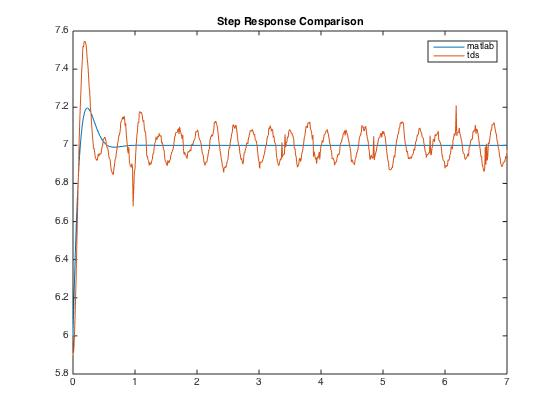
\includegraphics[scale=.4]{stepM1_T2}
            \caption{Step Response m1t2}
            \label{fig:stepM1_T2}
        \end{minipage}%
    \end{figure}
    \begin{figure}[H]
        \centering
        \begin{minipage}{.5\textwidth}
            \centering
            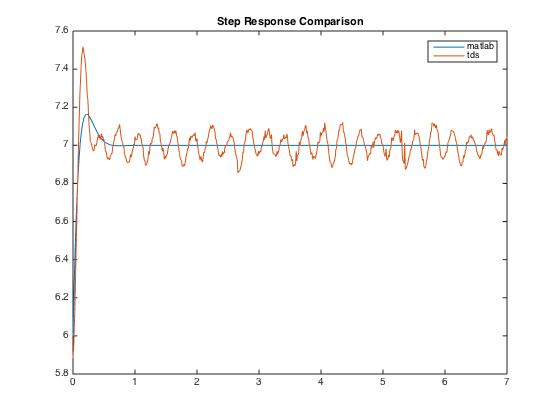
\includegraphics[scale=.4]{stepM1_T3}
            \caption{Step Response m1t3}
            \label{fig:stepM1_T3}
        \end{minipage}%
        \begin{minipage}{.5\textwidth}
            \centering
            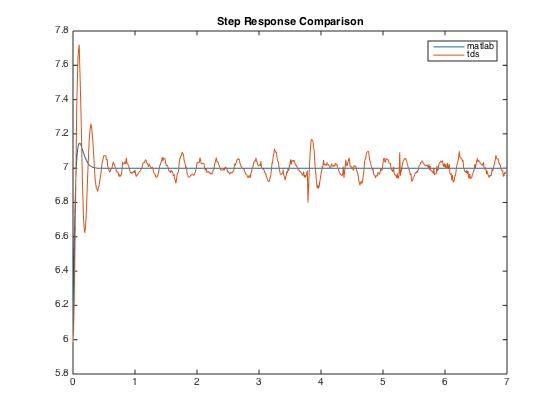
\includegraphics[scale=.4]{stepM1_T4}
            \caption{Step Response m1t4}
            \label{fig:stepM1_T4}
        \end{minipage}%
    \end{figure}
    \begin{figure}[H]
        \centering
        \begin{minipage}{.5\textwidth}
            \centering
            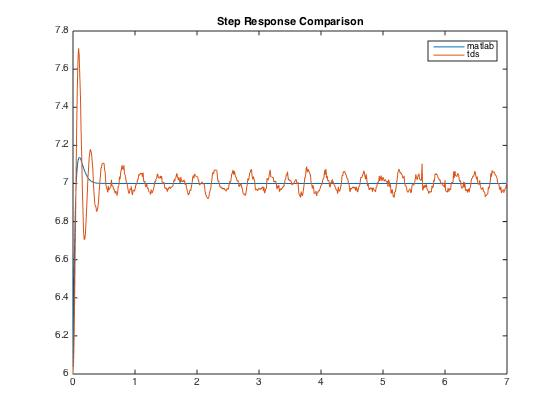
\includegraphics[scale=.4]{stepM1_T5}
            \caption{Step Response m1t5}
            \label{fig:stepM1_T5}
        \end{minipage}%
        \begin{minipage}{.5\textwidth}
            \centering
            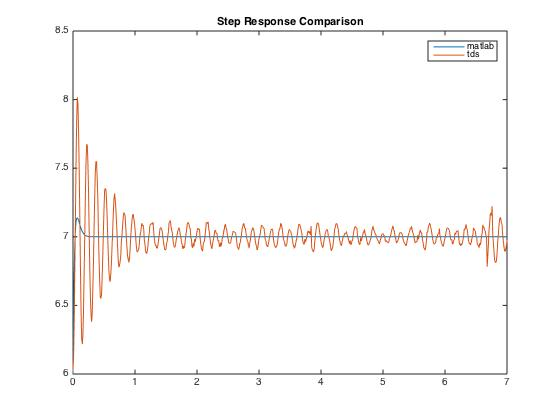
\includegraphics[scale=.4]{stepM1_T6}
            \caption{Step Response m1t6}
            \label{fig:stepM1_T6}
        \end{minipage}%
    \end{figure}
    \noindent Figures \ref{fig:stepM1_T1} through \ref{fig:stepM1_T6} show the plots of the matlab data and the collected experimental data for machine 1. Figures \textcolor{red}{add machine 4 plots}. From this information it is possible to calculate the actual rise time and overshoot of the system for different $K_I$ and $K_p$ values. Table \ref{table:actualStep} shows the calculated $t_r$ and $M_p$ using matlab's stepinfo function. \textcolor{red}{filtered data???}
    \begin{table}[H]
        \centering
        \begin{tabular}{|m{2cm}|m{2cm}|m{2cm}|m{2cm}|m{2cm}|m{2cm}|} 
            \hline
            matlab $t_r$ & mach1 $t_r$ & mach4 $t_r$ & matlab $M_p$ & mach4 $M_p$ & mach4 $M_p$\\ 
            \hline
            0.275 & 0 & 0 & 16.646 & 0 & 0 \\ 
            \hline
            0.09 & 0 & 0 & 19.58 & 0 & 0 \\ 
            \hline
            0.085 & 0 & 0 & 16.23 & 0 & 0 \\ 
            \hline
            0.039 & 0 & 0 & 14.67 & 0 & 0 \\ 
            \hline
            0.038 & 0 & 0 & 13.63 & 0 & 0 \\ 
            \hline
            0.025 & 0 & 0 & 3.916 & 0 & 0 \\ 
            \hline
        \end{tabular}
        \caption{$t_r$ and $M_p$ Comparison} \label{table:stepComp}
    \end{table}

    \subsection{Time Domain - Disturbance} \label{sub:dist}

    \subsection{Frequency Domain}

\section{PI Controller Design}

\end{document}